\documentclass[12.5pt]{scrartcl}

%\usepackage[romanian, english, ngerman]{babel}
\usepackage[T1]{fontenc}
\usepackage{lmodern}
\usepackage{amsmath}
\usepackage{amsfonts}
\usepackage{amssymb}
\usepackage{mathrsfs}
\usepackage{microtype}
\usepackage[utf8x]{inputenc}
\usepackage{graphicx}
\usepackage{setspace}
\usepackage{float}

%\linespread{1.5}
\usepackage{multirow}
\usepackage{tabularx}


\title{RoboFace}
\date{\vspace{-7ex}}
\begin{document} 
	\maketitle
	\thispagestyle{empty}
	
	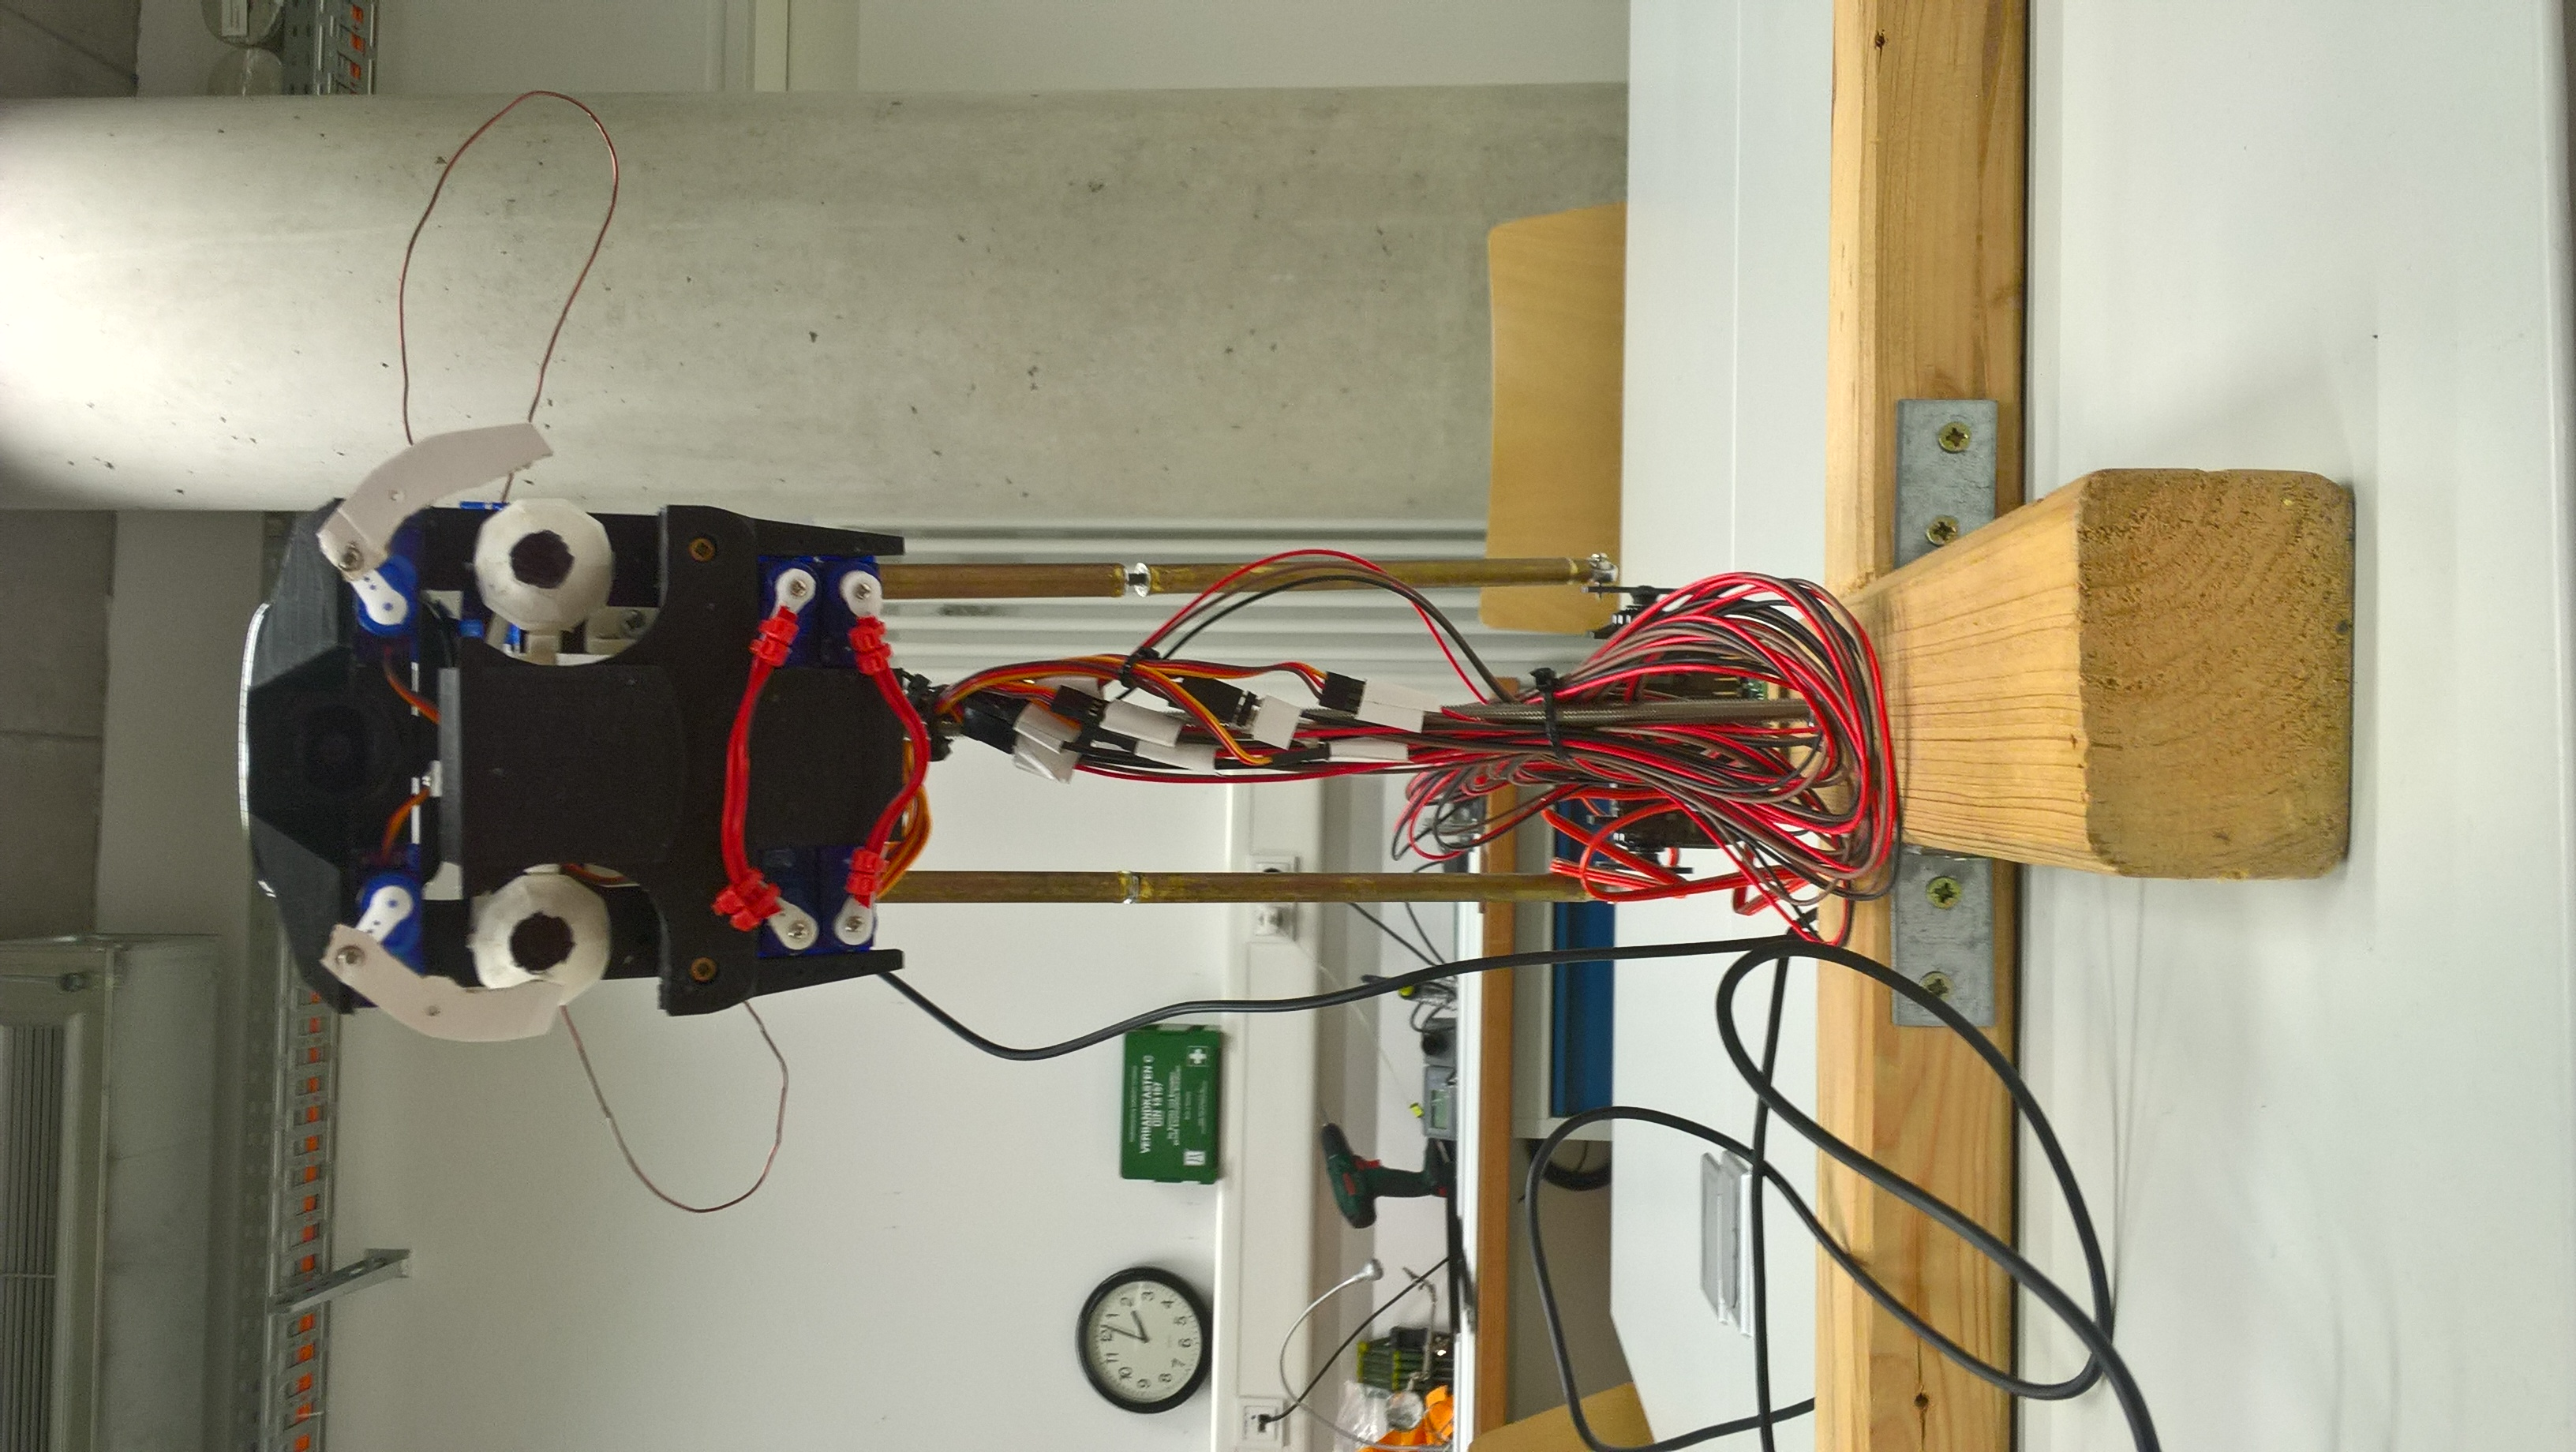
\includegraphics[width=0.88\linewidth]{images/roboFace}
	
	\begin{tabularx}{\textwidth}{Xl} 
		Kevin Kiefer      & Letitia Parcalabescu \\ 
		5. Semester Informatik  & 3. Semester Informatik \\ 
	\end{tabularx}
	
	Supervisors: Gero Plettenberg and Benjamin Reh
	
	\vspace*{8mm}
	\begin{center}
		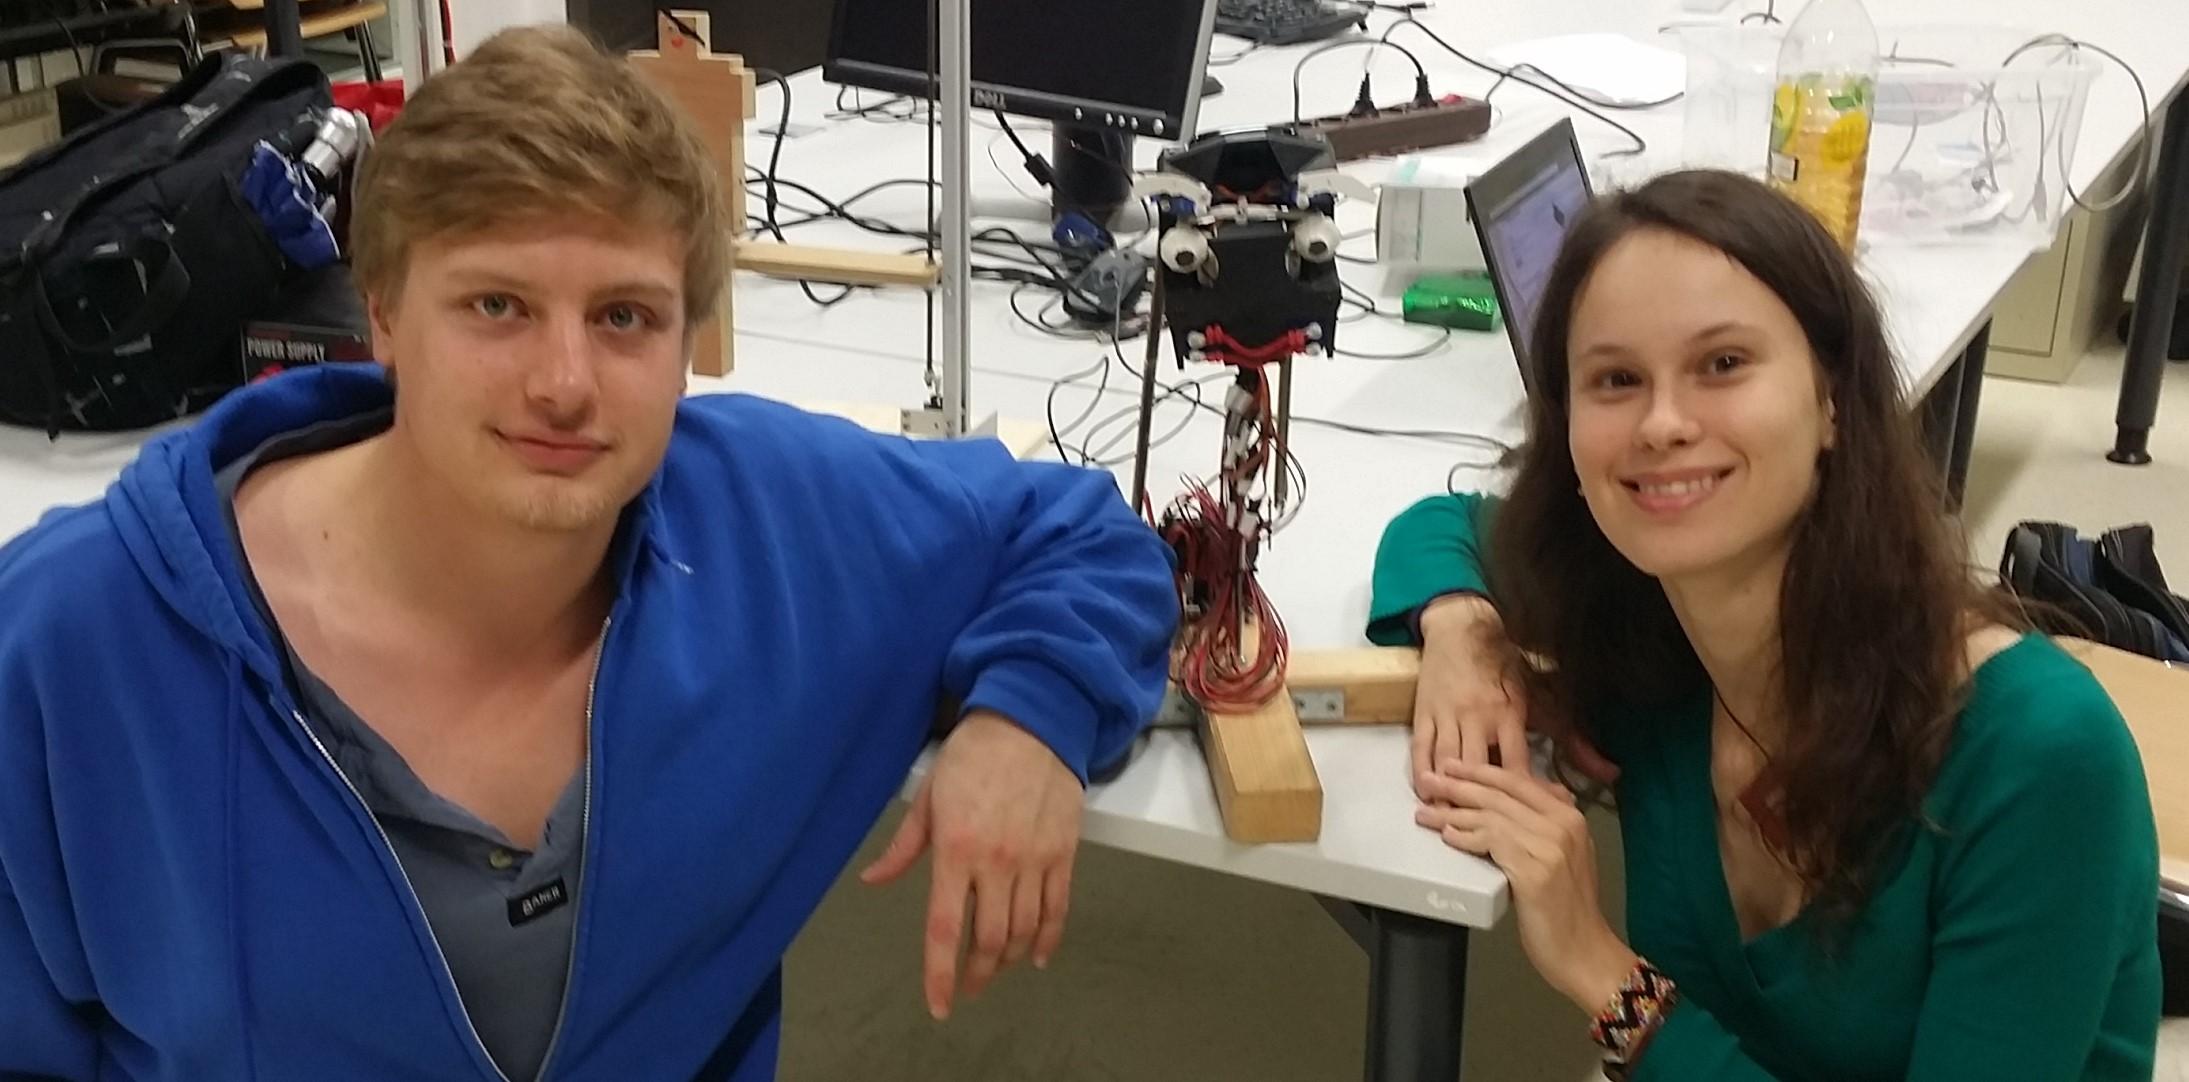
\includegraphics[width=0.88\linewidth]{images/faceEdited}
	\end{center}
	
	\section{Task:}
	Das vorhandene Robotergesicht, reagiert auf visuelle Reize mit akkustischen und mimischen Signalen. Dafür wurde eine Gesichtserkennung implementiert, dazu eine Sprachausgabe, die eine Reaktion auf das erkannte Gesicht ausdrücken soll. Das erkannte Gesicht wird von dem Roboter auch verfolgt, so dass Augenkontakt besteht.
	
	\section{Milestones:}
	\begin{itemize}
		\item Ende November: Überarbeitung der vorhandenen Codebase.
		\item Ende November: Gesichtererkennung
		\item Ende Dezember: Attributserkennung der vom Roboter betrachteten Gesichter
		\item Ende Dezember: Sprachausgabe
		\item Anfang Januar: Gesichtstracking
	\end{itemize}

	\section{Setup guide for the robot}
	\subsection{Hardware}
	\subsection{Software}
	\subsection{Funktionsweise der Gesichtserkennung - Die Magie hinter neuronalen Netzen}
	\subsubsection{Architektur}
	\begin{enumerate}
		\item 	32 of neurons in each convolutional layer
		\item Activations: Relu
		\item 9 x 9 convolution $\rightarrow$ Max Pooling
		\item	7 x 7 convolution $\rightarrow$  Max Pooling
		\item	5 x 5 convolution $\rightarrow$  Max Pooling
		\item	3 x 3 convolution $\rightarrow$  Max Pooling
		\item	3 x 3 convolution $\rightarrow$  Max Pooling
		\item	Dropout(0.25)
		\item	512 Dense
		\item	Dropout(0.5)
		\item	13 Dense
		\item	Sigmoid
		\item	Binary Crossentropy
		\item	Adadelta optimiser
		\item Overall: 125,709 parameters
	\end{enumerate}
	\subsubsection{Trainingsdatensatz}
	http://mmlab.ie.cuhk.edu.hk/projects/CelebA.html
	
	202.599 Bilder, 10.177 Identitäten, 40 Attribute pro Bild
	
	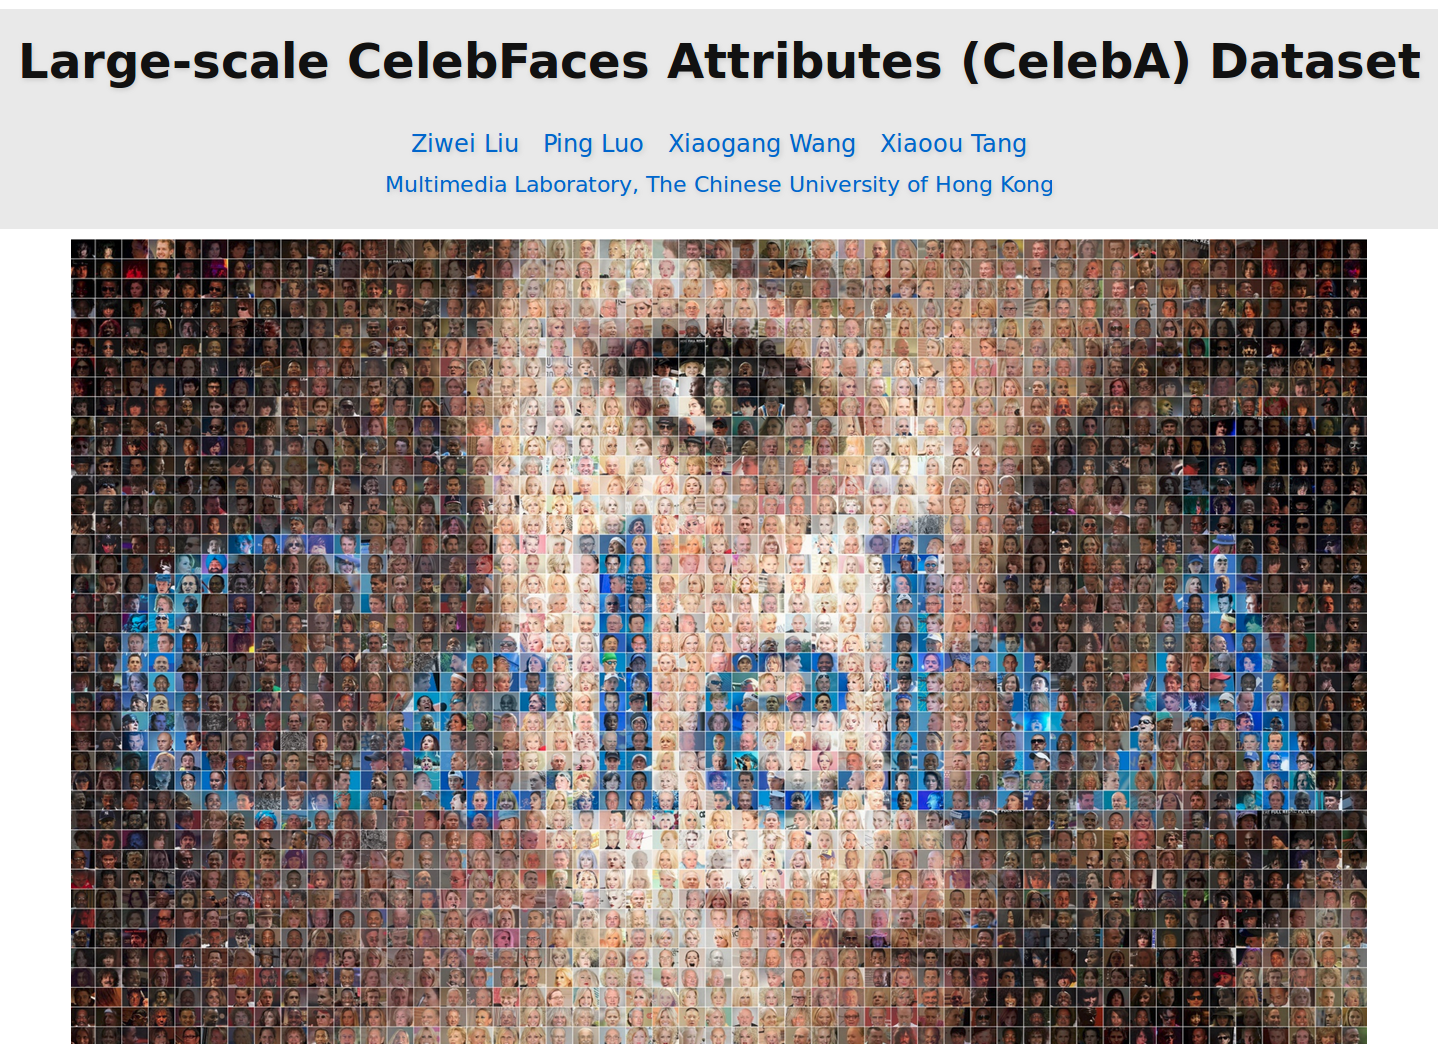
\includegraphics[width=0.88\linewidth]{images/CelebA} \\
	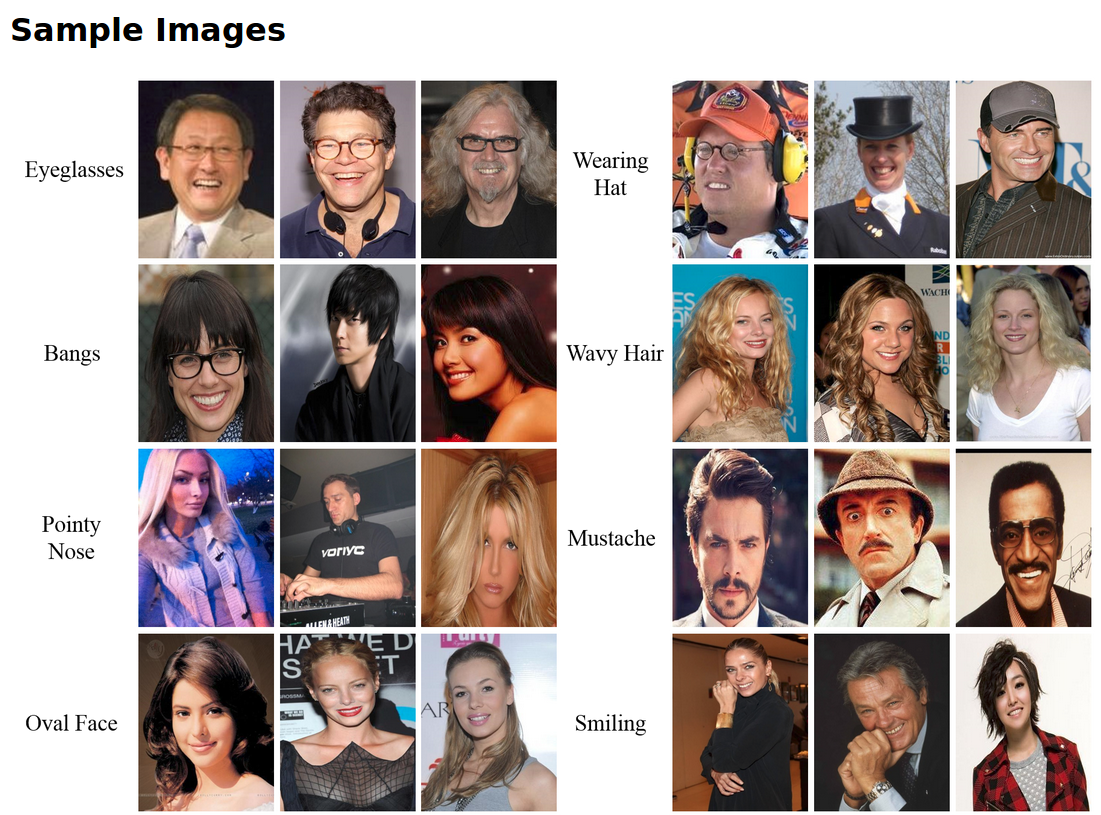
\includegraphics[width=0.88\linewidth]{images/CelebAExamples}
	
	Wähle 13 Attribute aus den 40 die zur Verfügung stehen.
		\begin{enumerate}
			\item Black Hair
			\item Blond Hair
			\item Brown Hair
			\item Eyeglasses
			\item Gray Hair
			\item Male
			\item Mouth Slightly Open
			\item No Beard
			\item Smiling
			\item Straight Hair
			\item Wavy Hair
			\item Wearing Earrings
			\item Wearing Lipstick
		\end{enumerate}
	\subsubsection{Normalisierung der Daten}
	NOT! Obwohl hier die Trainingkurven sehr gut aussehen, täuschen diese auf dem ersten Blick. Wenn man das generalisrieungsvermögen des Netzes untersucht, stellt man fest, dass die \\
	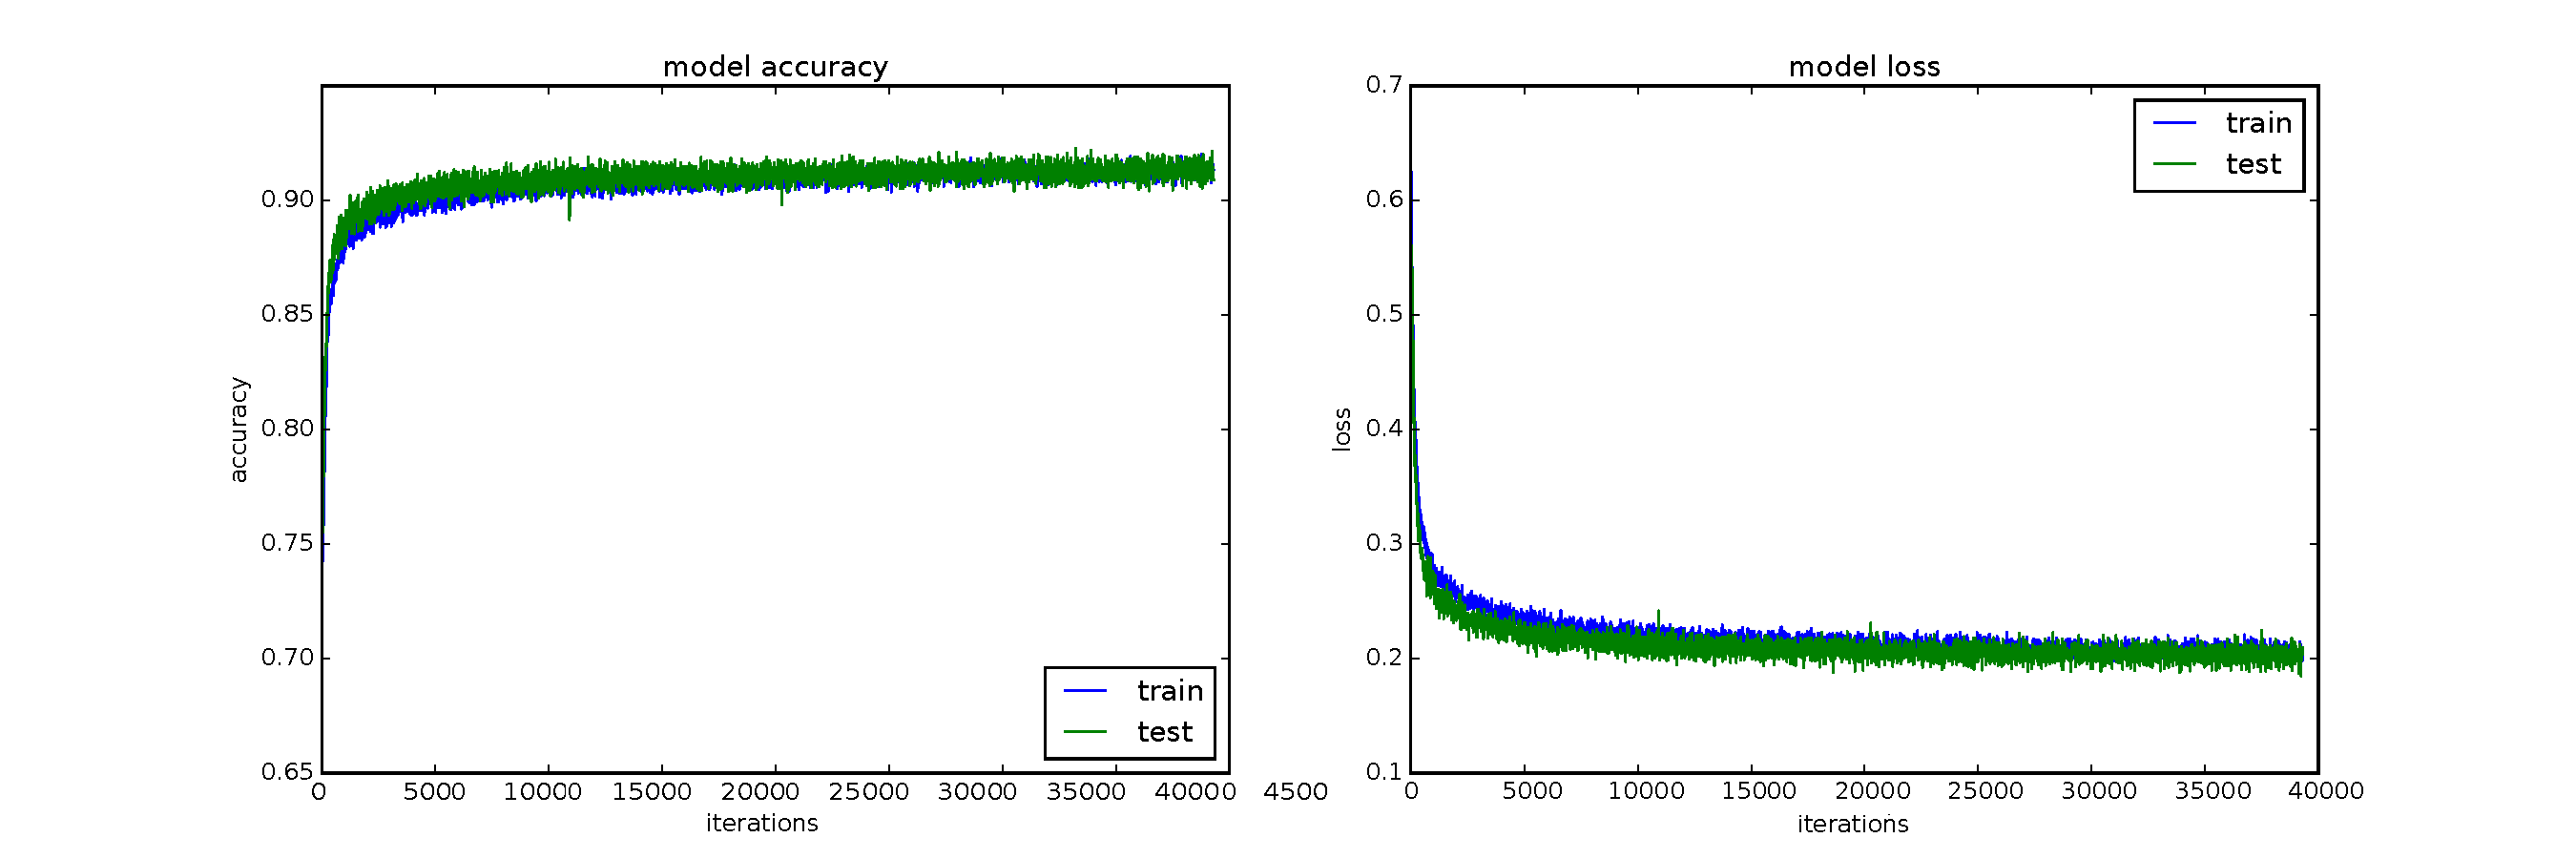
\includegraphics[width=\linewidth]{images/lossBad}\\
	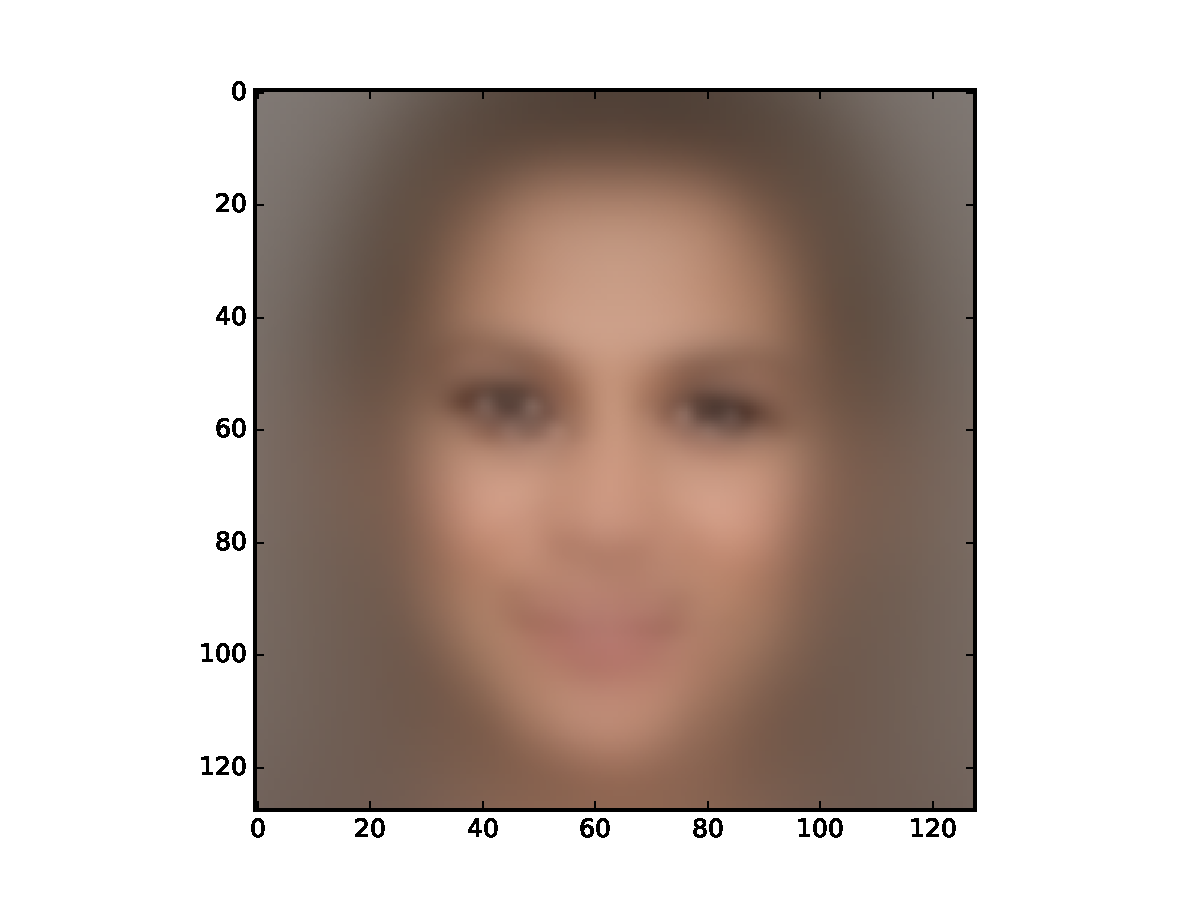
\includegraphics[width=0.88\linewidth]{images/meanFace}\\
	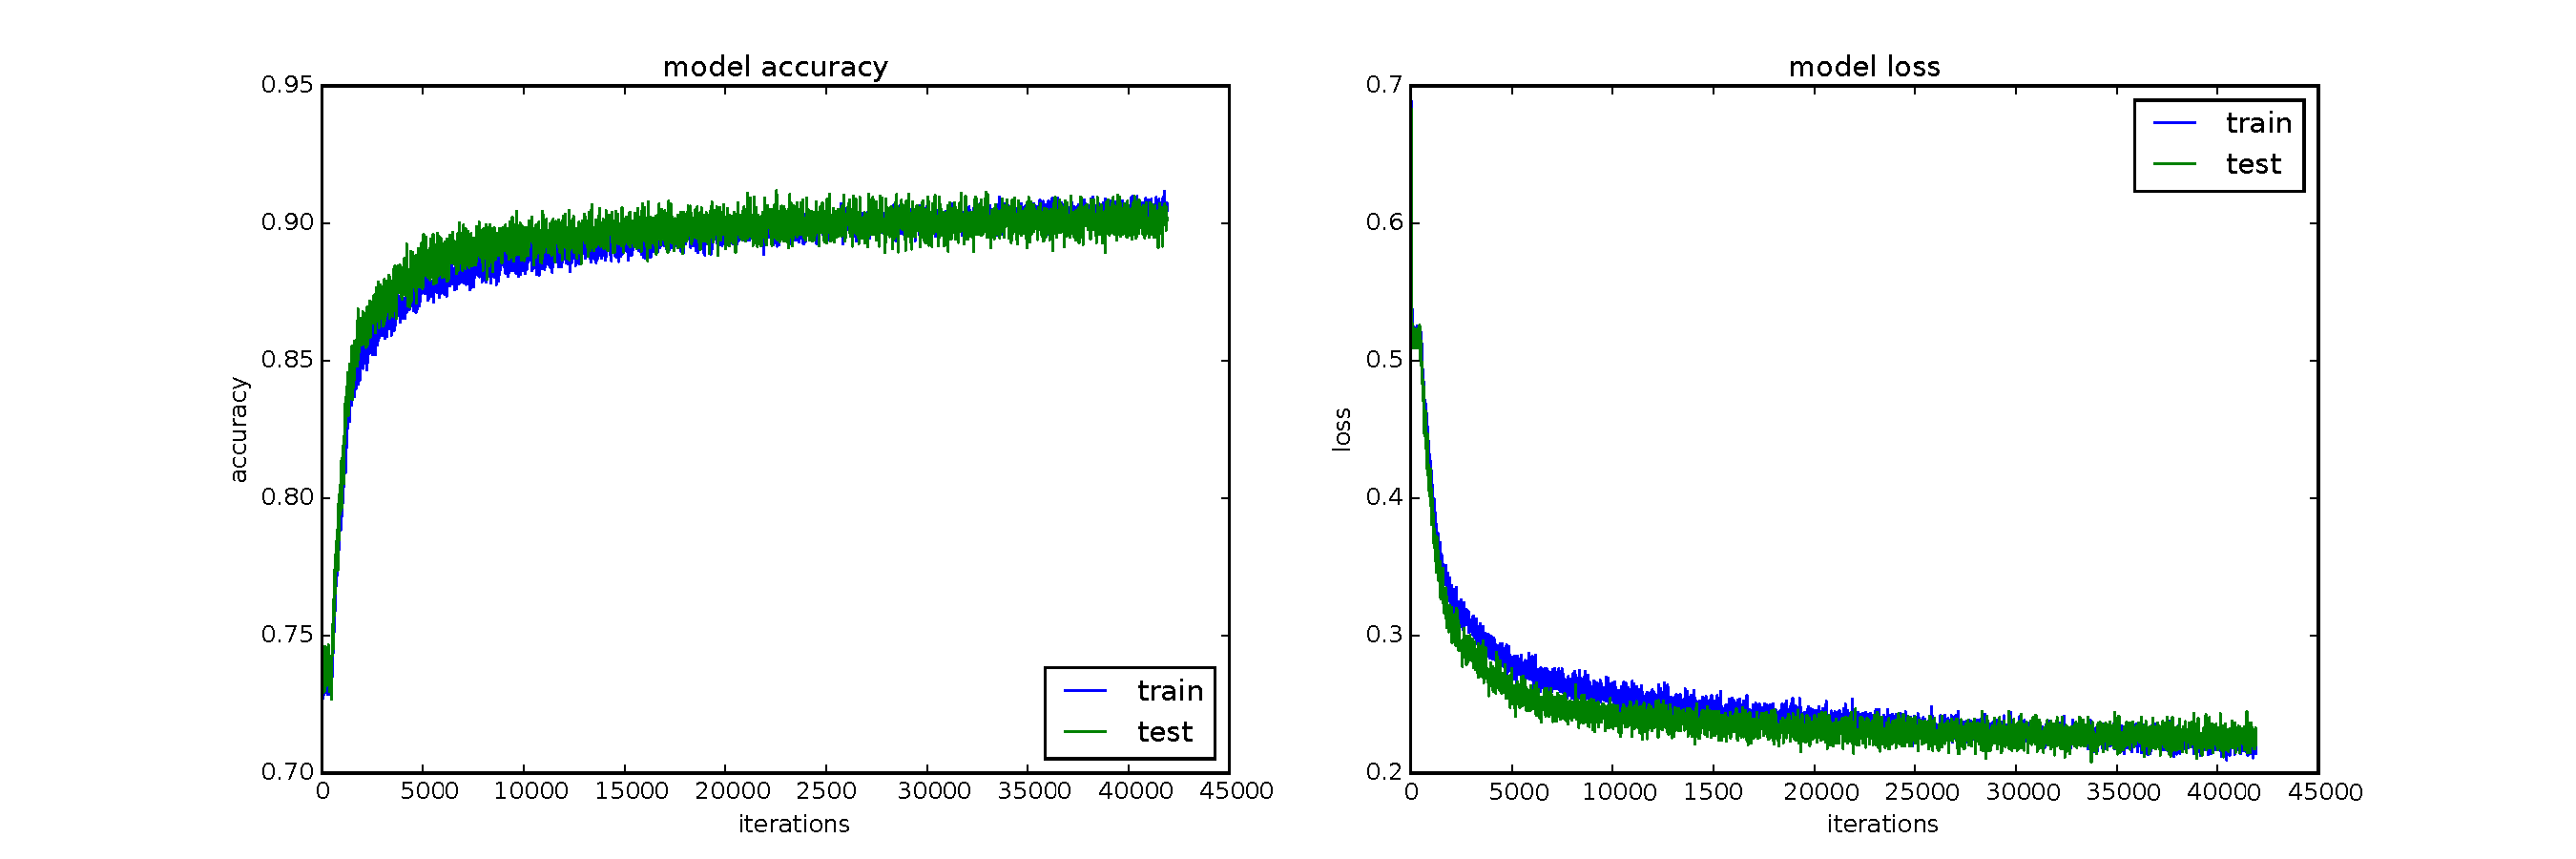
\includegraphics[width=\linewidth]{images/lossGood}\\
	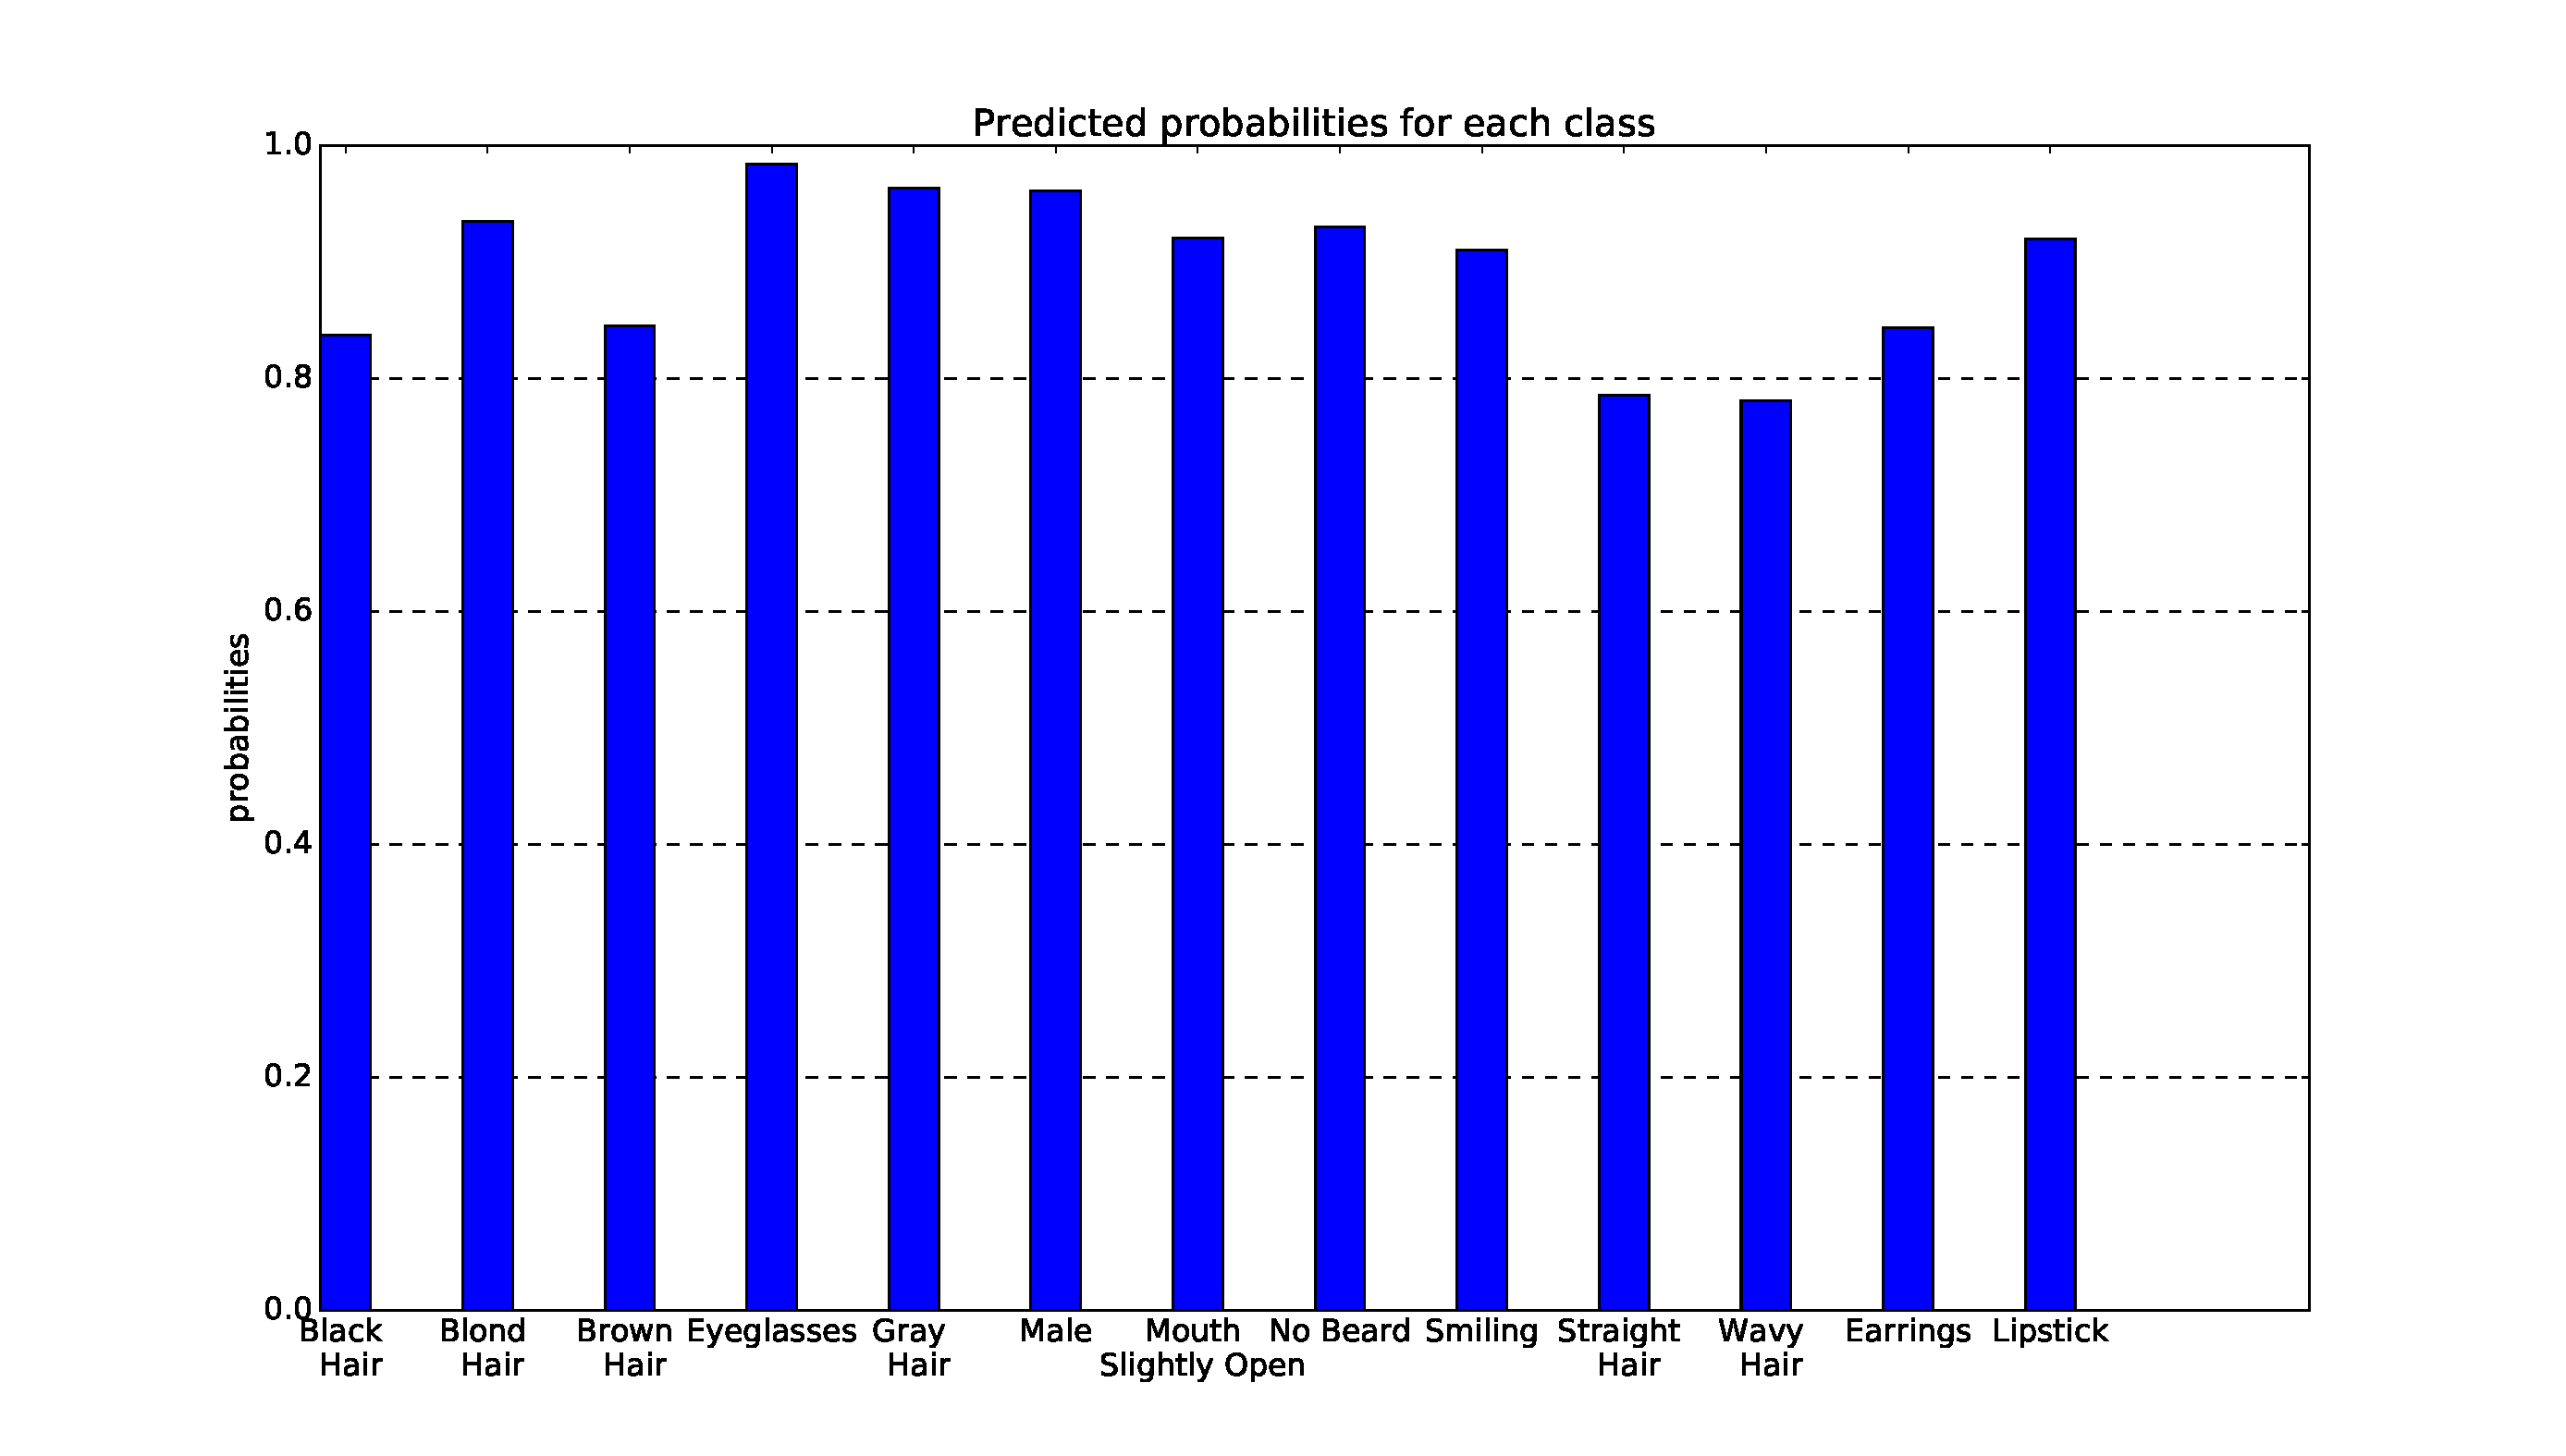
\includegraphics[width=0.88\linewidth]{images/accuracy_on_classes}
	\section{Ausblick}
	Verbeserung der Hardware
	\section{Quellcode}
	github Link
	
\end{document} 